\section{Joint protocol, convergence and paired network validation}
\label{sec:extendedvalidation}
The extension follows the order instrument verification, bounded spin-bath convergence, paired simulator pilot and larger simulator study. Numerical prerequisites are checked before the next workload starts. These gates authorize the following \emph{software control}, not an experimental or new-material prediction. All configurations and thresholds are retrospective; no new hardware measurement is included.

\subsection{Time-dependent fidelity, signal retrieval and readout noise}
Seven hypothetical instruments cover identity, complete loss, background-only acceptance, dephasing with loss, thermal/background noise, biased background and noise-dominated retrieval. Eight storage ages span 0--100 ms. A separately implemented Liouvillian and matrix-unit reference constructs the complete qubit-to-qutrit map in Eq.~\eqref{eq:detectedinstrument}; it does not reuse the lab's Kraus construction. The checks include the full Choi matrix, six Pauli-state outputs, average fidelity, signal/noise/acceptance probabilities, complete positivity and trace preservation. All \ProtoPoints{} channel-age points and \ProtoProbes{} state probes pass at tolerance $10^{-10}$; the maximum numerical discrepancy is \ProtoError{}.

\begin{figure}[tbp]
\centering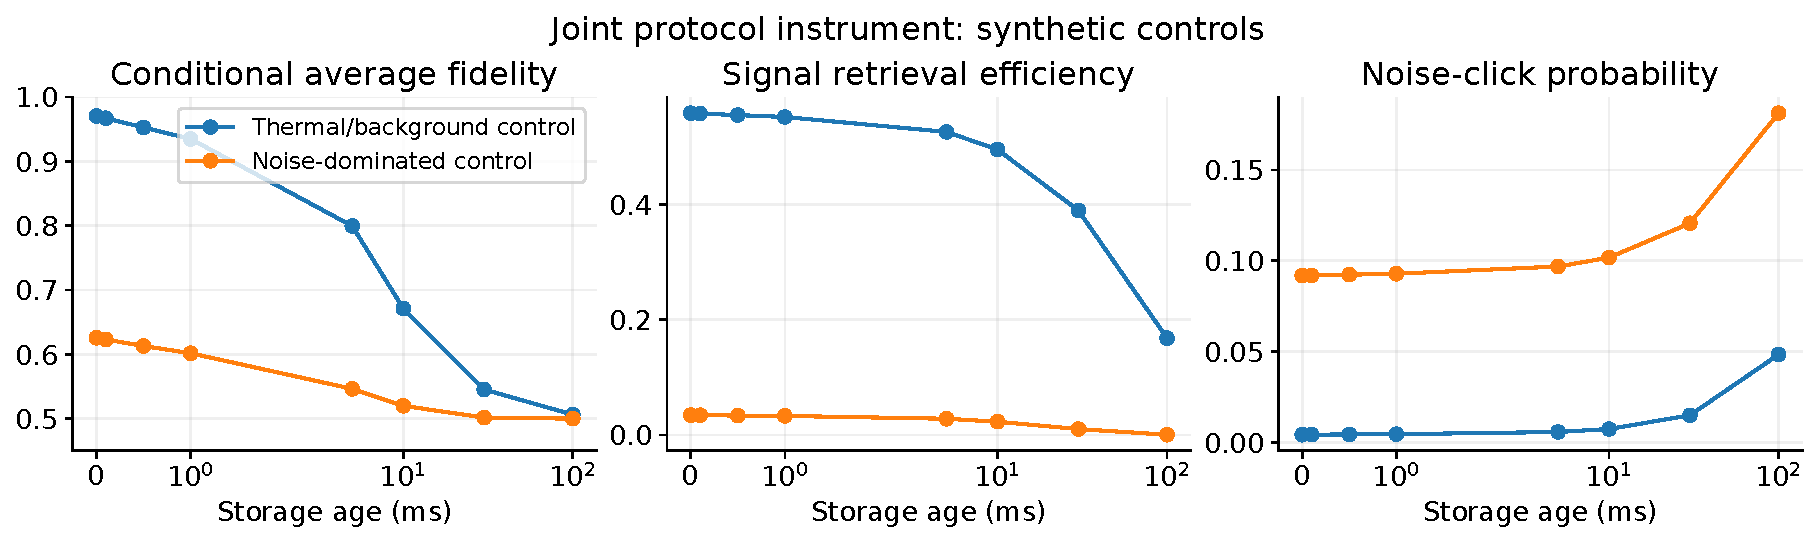
\includegraphics[width=\linewidth]{figures/validation_extension/protocol_joint.pdf}
\caption{Joint instrument controls, generated from retained numerical results. Signal efficiency, accepted noise and conditional fidelity vary together under the supplied rates. Background-only clicks do not become signal efficiency; a noise-dominated accepted output can approach average fidelity $1/2$. Curves are synthetic effective models, not experimental fits. The horizontal scale is linear near zero and logarithmic at longer ages.}
\label{fig:jointprotocol}
\end{figure}

An audit of the bundled PR2026 heralded-photon arrays retains nine ages with efficiency, noise and signal--idler $g^{(2)}$, together with source errors. They have no matching qubit-fidelity series. The 0.9 $\mu$s source/article clock difference remains unresolved; noise per herald cannot be assumed to equal a vacuum false-click probability. Neither Teller's fixed operating point nor Bradley's nuclear-spin observables supplies the missing optical time series. Joint \emph{experimental} validation therefore remains inconclusive, with no fidelity inferred from $g^{(2)}$ or imported from another device. The pending data contract requires matched state/tomography, retrieval and background-only counts, common trial denominators and clocks, detector windows, photon statistics, pulse/field/temperature conditions, and uncertainty/covariance definitions.

\subsection{Bounded noncommuting spin-bath convergence}
The nested synthetic bath has 2, 4, 6 and 8 $^{13}$C spins, maximally mixed initialization and central projections $m=\pm1/2$. Noncommuting transverse hyperfine terms accompany longitudinal couplings and explicit nuclear-pair tensors. Ideal control has 0, 1 or 4 CPMG pulses over 0--0.4 ms. An independent spectral propagator is compared with matrix exponentials, followed by Strang-step, CCE-order, pair-cutoff, bath-size and time-grid studies. There are \ConvCalls{} actual coherence solver calls and \ConvRows{} diagnostic rows; final comparisons pass all six controls (Table~\ref{tab:validationconvergence}). Lower-level failures remain in the archived table and Fig.~\ref{fig:spinconvergence}.
\begin{table}[tbp]\centering\small
\begin{tabular}{p{.29\linewidth}p{.25\linewidth}rr}\toprule Control & Final comparison & Maximum error & Tolerance\\\midrule
Matrix exponential / spectral & 4-spin reference & \ensuremath{1.444\times10^{-15}} & \ensuremath{1.000\times10^{-10}}\\
Strang substeps & 128 substeps & \ensuremath{2.332\times10^{-5}} & \ensuremath{1.000\times10^{-4}}\\
CCE order & Order 4; 4 spins & \ensuremath{4.132\times10^{-10}} & \ensuremath{1.000\times10^{-3}}\\
Pair cutoff & 40 angstrom; 4 spins & \ensuremath{4.132\times10^{-10}} & \ensuremath{1.000\times10^{-3}}\\
Bath size & 6 to 8 spins & \ensuremath{1.452\times10^{-8}} & \ensuremath{1.000\times10^{-3}}\\
Mean $|L|$ integration & 129 to 257 points & \ensuremath{1.950\times10^{-6}} & \ensuremath{1.000\times10^{-4}}\\
\bottomrule\end{tabular}
\caption{Final convergence diagnostics over 0--0.4 ms, taking the maximum over 0, 1 and 4 ideal pulses. Solver, CCE and cutoff errors use the exact four-spin reference; bath-size and time-grid errors compare adjacent nested levels. The time-grid metric is mean absolute coherence, not every revival extremum or an inferred lifetime.}\label{tab:validationconvergence}\end{table}


\begin{figure}[tbp]
\centering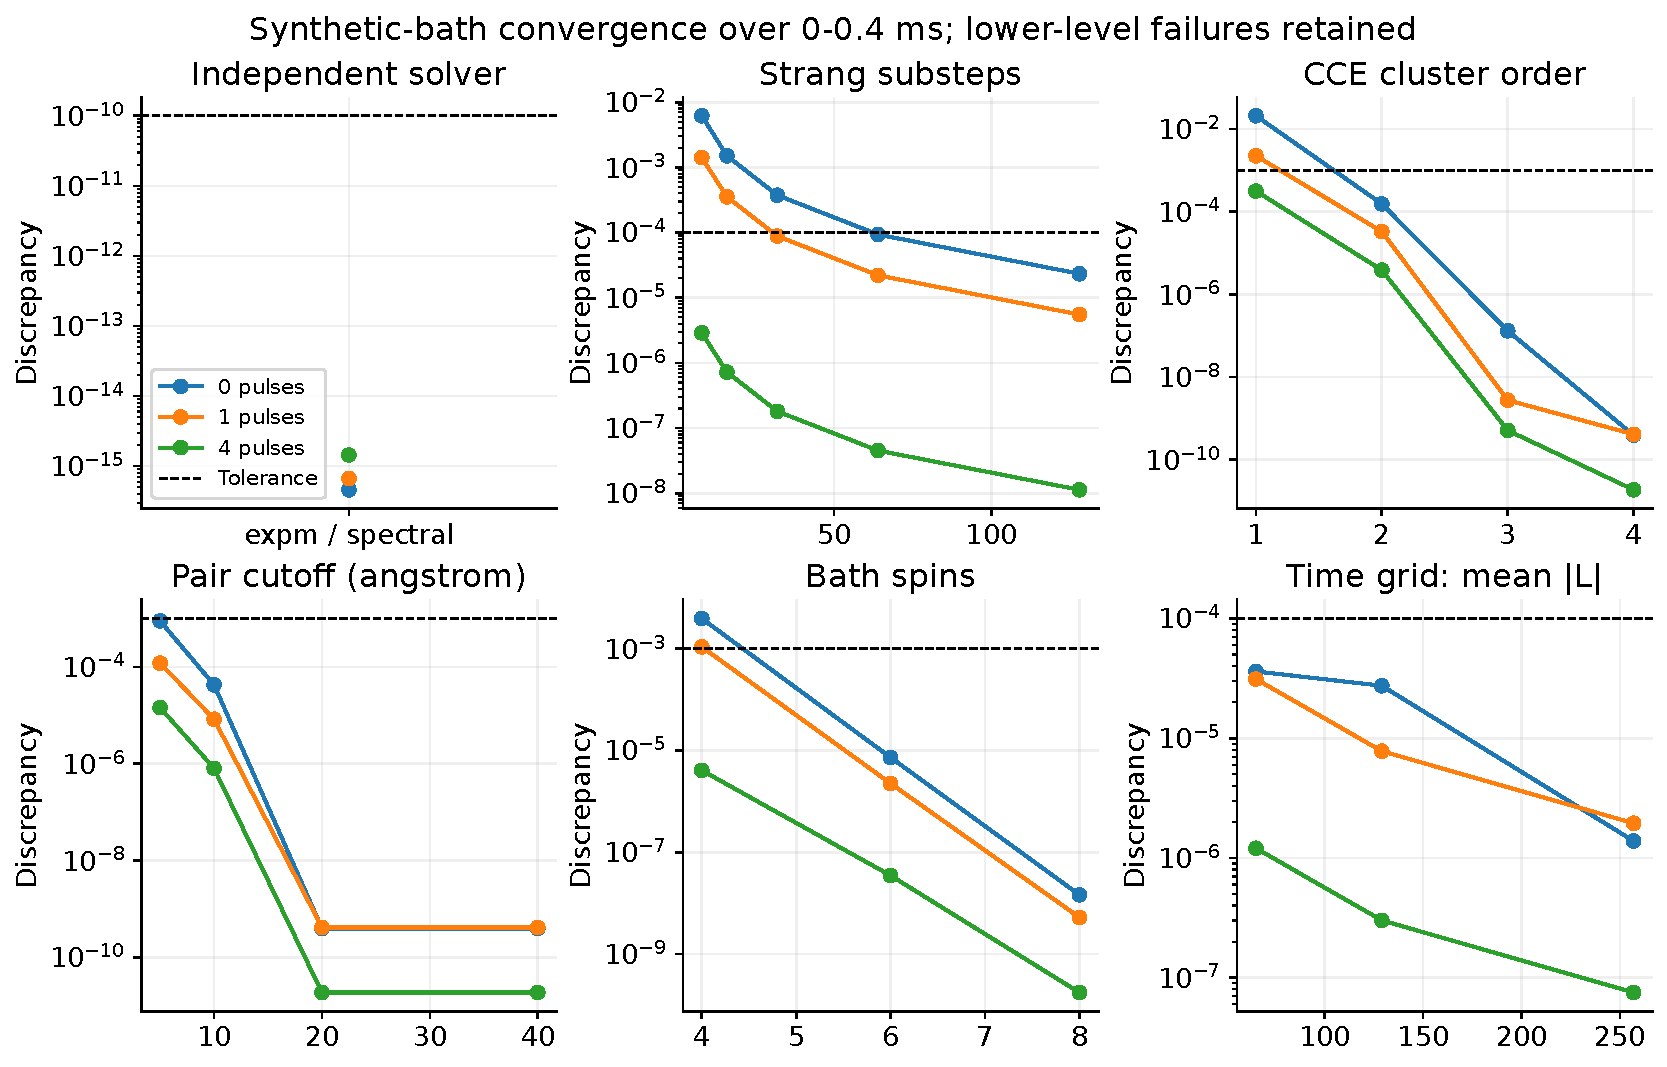
\includegraphics[width=\linewidth]{figures/validation_extension/spin_convergence.pdf}
\caption{All six convergence controls for the supplied noncommuting synthetic baths; dashed lines are declared numerical tolerances. Bath-size and time-grid points compare adjacent levels and omit the first level, which has no preceding comparator. Other panels use the independent/exact four-spin reference. The time-grid ordinate is an error in integrated mean $|L|$. Ideal-pulse propagation convergence is not a pulse-shape or pulse-error study.}
\label{fig:spinconvergence}
\end{figure}

The supplied outer couplings deliberately decrease rapidly. This is not a material lattice, measured hyperfine distribution or disorder ensemble. Consequently, the small last-step error cannot authorize a larger bath or longer observation window for another material. PyCCE now receives all explicitly supplied pair tensors, including zero tensors where relevant; otherwise it can generate dipolar interactions for unspecified pairs. The field/isotope Zeeman convention is checked against the exact reference. The Supplement records the full Hamiltonian recipes and unit conversions.

Profiles explicitly declaring \code{prediction\_purpose: material\_prediction} now require a passing certificate with a matching profile-content hash, five converged refinement axes, error below the declared tolerance, a valid time interval and independent physical-model review. Hypothetical evidence cannot authorize such a prediction. This checks declared evidence and identity, not the scientific validity of a self-issued certificate; legacy profiles without that purpose label continue to run without receiving a new material endorsement. No material certificate is issued by this study.

\subsection{A second native simulator and the larger paired study}
SeQUeNCe 1.2.0 runs its native event kernel and density manager. QuNetSim 0.1.2~\cite{qunetsim} runs its native hosts, quantum connections, packet queues and acknowledgements with a new protocol-specific QuTiP density backend. The latter preserves joint states during transmission and consumes retrieved/lost qubits; it is not QuNetSim's stock EQSN backend. An independent matrix-unit reference checks local and joint channel action. These are two executed simulator stacks, rather than two channel descriptions in one simulator.

The stacks share external logical ages and three separate seeded streams for heralding and the two readouts. Sixteen parameter combinations use background rates 0 and 5000 s$^{-1}$, ages 0, 1, 10 and 30 ms, and herald probabilities 0.25 and 0.75. Attempts are spaced by 40 ms and the model ensemble Bell-fidelity gate is 0.8. Quality qualification uses this ensemble gate, not unobservable per-trial signal/noise labels. The pilot and larger study use separate fresh processes because QuNetSim's global network instance is not restarted within a completed worker.
\begin{table}[tbp]\centering\small
\begin{tabular}{lrrrrr}\toprule Study & Seeds & Pairs of runs & Arm runs & Trials/run & Trials, both arms\\\midrule
Pilot & 3 & 48 & 96 & 32 & 3\,072\\
Larger & 8 & 128 & 256 & 512 & 131\,072\\
\bottomrule\end{tabular}
\caption{Actual native simulator work counts. Each parameter/seed combination is executed once per simulator. Paired shared traces test implementation agreement; seeds are the independent Monte Carlo clusters. Pilot and larger stages are separate processes and use different seeds.}\label{tab:validationcrosssim}\end{table}


After the pilot passes, the larger study completes \LargerRuns{} arm runs and \LargerAttempts{} trials across both simulators. All \LargerPairs{} paired comparisons have identical branch counts and logical trace hashes; the maximum difference between mean joint density matrices is \LargerError{}, below $10^{-10}$. SeQUeNCe executes \NativeEvents{} native events and QuNetSim transfers \NativeTransfers{} quantum packets. No arm fails. Paired runs have identical random inputs by design; their agreement is implementation verification, not independent experimental replication.

\begin{figure}[tbp]
\centering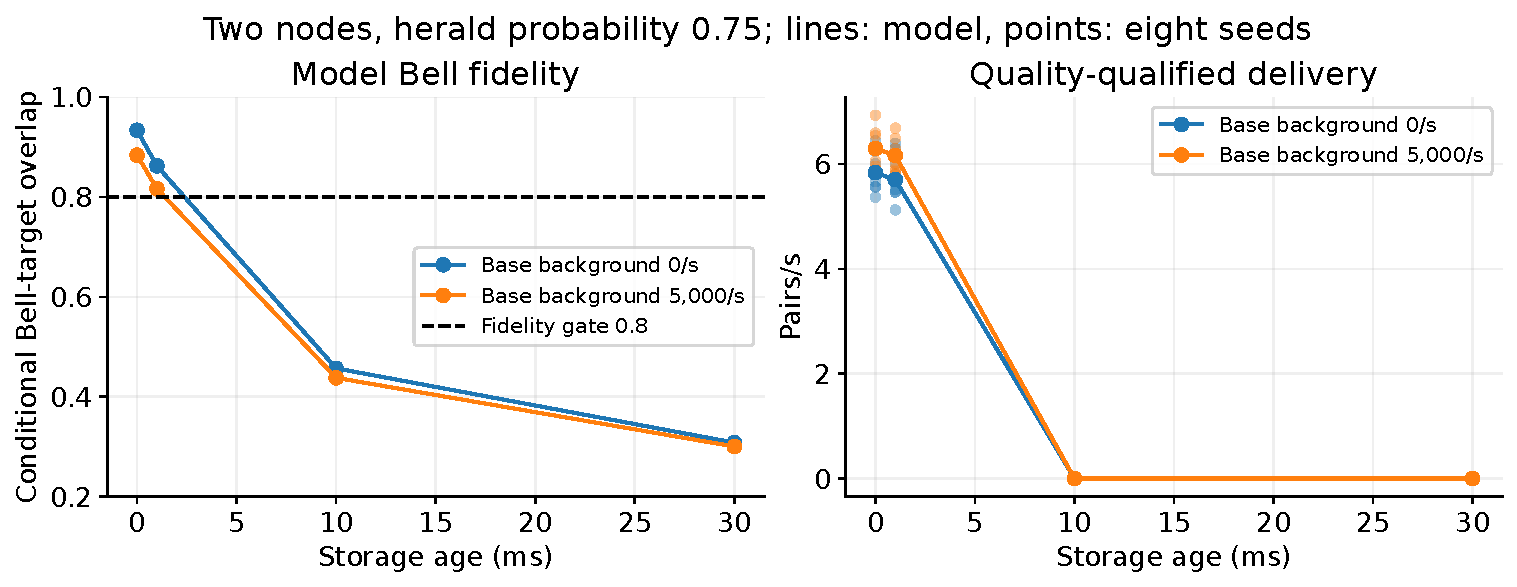
\includegraphics[width=\linewidth]{figures/validation_extension/crosssim_larger.pdf}
\caption{Larger-study ensemble Bell fidelity and quality-qualified pair rate at herald probability 0.75. Lines show the supplied model expectation at sampled ages; points show all eight seed-cluster outcomes. Acceptance can increase with background while fidelity decreases, so accepted-pair counts alone are insufficient. Eight seeds are eight independent Monte Carlo clusters per parameter combination; no cross-parameter independence, coverage, power or speedup is inferred. Both simulators give the same paired counts.}
\label{fig:crosssimlarger}
\end{figure}

QuNetSim uses real-time worker scheduling~\cite{qunetsim}, which is not equated with a physical network clock here. The common logical trace is an externally imposed test input; agreement of its hash does not cross-validate native physical latency. The workload has two nodes and one slot, and omits routing, swapping, contention, finite fiber propagation and detector double clicks. This boundary is narrower than latency-and-resource cross-validation such as Chung et al.~\cite{chung}. Runtime records are retained as execution metadata without a comparative performance claim.

\subsection{Replay and current test scope}
A fresh denied-network replay reproduces \ReplayRecords{} JSON records and \ReplayArrays{} exact random-trace arrays, including every archived native run. Lab/evaluation/configuration fingerprints match; the absolute and relative numerical tolerance is $10^{-10}$. Each ZIP archive's SHA-256 is verified before its contents are compared. Timestamps, environment/runtime metadata and archive-container bytes are excluded from scientific equality. The current extension environment runs \LatestTests{} tests: \LatestPass{} pass and \LatestSkip{} optional PySCF/MaxwellBloch tests are skipped. These counts describe that environment; they do not replace the earlier full-environment test snapshot. Historical system stages 1--4 also preserve their full scientific payloads under an explicit cross-revision comparison. All checks are author-operated, not colleague-led independent scientific review.
